\section{Results}
\label{sec:results}
We organize the results around the three predictions from Section~\ref{sec:mechanism}: whether the no-skill anchor changes a two-arm verdict, where a targeted procedure is binding rather than ceiling-limited, and whether unchanged procedures retain direction on compatible future releases. Endpoints are the independent units; repeats measure execution robustness only.

\subsection{The third arm changes the scientific verdict}
\label{sec:falsepositive}
The clearest justification for the design is a negative result. On DeepSeek C3-R cutoff, the targeted procedure succeeds on 100\% of endpoint-repeat observations and the matched generic helper on 72\%. A conventional T-versus-G comparison would therefore report a +28-point benefit. The no-skill agent, however, is also at 100\%. Thus $\widehat{\Delta}_{T-G}=+28$ points but $\widehat{\Delta}_{T-N}=0$, and Definition~1 classifies the cell as \emph{no repair}.

The frozen G1 helper explains why this is a plausible failure mode for a generic control: it validates schema-compatible evidence but is deliberately forbidden from comparing release dates with the cutoff, so it can foreground both an admissible release and a post-cutoff distractor. T1 performs the missing cutoff operation, but in this cell it only restores the behavior of the original agent. The same pattern appears more weakly in DeepSeek C4-R, while Kimi cutoff is at ceiling. The three-arm design therefore does more than reduce variance: it prevents a generic-arm deficit from being promoted into a procedure-repair claim.

A zero-call r9 audit further shows that T--G is not explained by unequal helper availability: targeted and generic helpers are each forced exactly once in all 442 retained rows of their respective arms, versus 0/442 in no-skill; condition position has no detectable success association in any arm ($p>.65$), and targeted prompts are 18.85 input tokens shorter on average than their exact generic counterparts. These diagnostics close simple invocation/order/length explanations for T--G. They do not turn N into a resource-matched arm, because N executes no helper, and they do not make G behaviorally neutral. The present T--N contrast should therefore be read as incremental value over the original agent, while a neutral-helper candidate G$_0$ remains the prospective test of whether the targeted operation adds value beyond behaviorally neutral extra computation.

\begin{figure}[t]
\centering
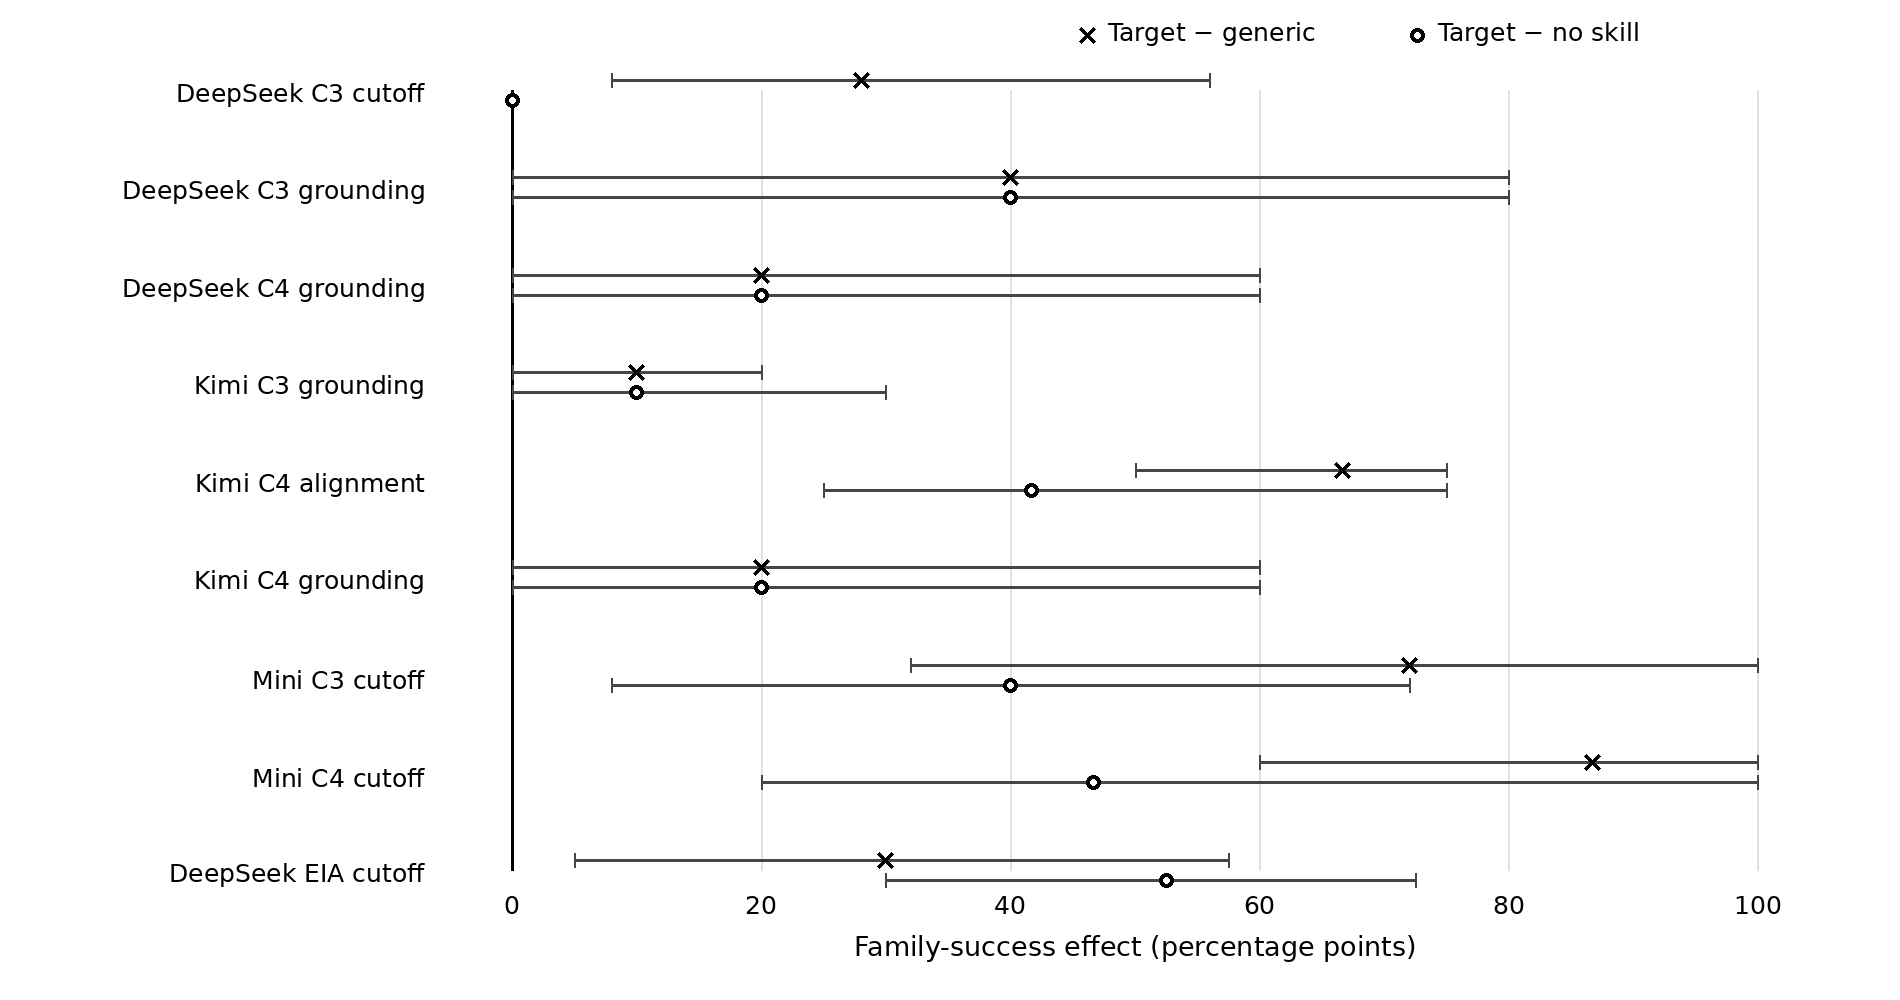
\includegraphics[width=0.96\linewidth]{figures/fig2_regime_effects.png}
\caption{Temporal-procedure effects are regime-dependent. Circles compare targeted with the original no-skill agent; crosses compare targeted with the matched generic helper. Horizontal bars show endpoint-bootstrap 95\% intervals. DeepSeek C3 cutoff illustrates the identification point: T$>$G but T$=$N, so the apparent two-arm gain is not a repair. EIA denotes the frozen post-review energy validation.}
\label{fig:regimes}
\end{figure}

\begin{table}[t]
\centering
\small
\setlength{\tabcolsep}{3.2pt}
\begin{tabular}{llrrrrr}
\toprule
Model / split & Family & N0 & Generic & Target & $\Delta_{T-G}$ & $\Delta_{T-N}$ \\
\midrule
DeepSeek C3-R & Cutoff & 100 & 72 & 100 & +28 & 0 \\
DeepSeek C3-R & Align & 100 & 100 & 100 & 0 & 0 \\
DeepSeek C3-R & Ground & 20 & 20 & 60 & \textbf{+40} & \textbf{+40} \\
DeepSeek C4-R & Cutoff & 100 & 87 & 100 & +13 & 0 \\
DeepSeek C4-R & Align & 100 & 100 & 100 & 0 & 0 \\
DeepSeek C4-R & Ground & 40 & 40 & 60 & \textbf{+20} & \textbf{+20} \\
\midrule
Kimi repl. C3-R & Cutoff & 100 & 100 & 100 & 0 & 0 \\
Kimi repl. C3-R & Align & 100 & 100 & 100 & 0 & 0 \\
Kimi repl. C3-R & Ground & 30 & 30 & 40 & +10 & +10 \\
Kimi repl. C4-R & Cutoff & 100 & 100 & 100 & 0 & 0 \\
Kimi repl. C4-R & Align & 58 & 33 & 100 & \textbf{+67} & \textbf{+42} \\
Kimi repl. C4-R & Ground & 60 & 60 & 80 & \textbf{+20} & \textbf{+20} \\
\bottomrule
\end{tabular}
\caption{Registered DeepSeek and provenance-clean Kimi replication family success (percent). DeepSeek has five repeats; Kimi retains four. Bold entries improve over both controls. Repeats are not treated as independent endpoint samples.}
\label{tab:primaryrep}
\end{table}

\subsection{Grounding is a binding repair when the original agent has headroom}
DeepSeek gives the cleanest primary-track positive case. Across five C3-R grounding endpoints and five repeats, N0 and G3 each succeed on 5/25 endpoint-repeat observations while T3 succeeds on 15/25: 20\%, 20\%, and 60\%, respectively. Hence both contrasts are +40 points, with the same direction in every repeat. At the endpoint level, targeted-minus-generic has two wins, three ties, and no losses; its endpoint-bootstrap 95\% interval is [0,80] points. Kimi shows a smaller C3-R directional gain of 10 points over both controls.

Held-out grounding is directionally consistent but low-resolution. Across all C4-R grounding endpoints, DeepSeek moves from 40\% under either control to 60\% with T3, and Kimi from 60\% to 80\%. On the two pre-registered same-domain held-out endpoints, both models show a descriptive 50-point targeted gain over both controls. Cross-domain grounding, however, shows no incremental targeted effect. We therefore interpret the evidence as future-period reuse within the compatible grounding regime, not broad cross-domain portability.

\subsection{Cutoff repair appears in non-ceiling regimes and disappears at ceiling}
The initial exploratory mini-model stress exposes cutoff headroom that is absent from the primary DeepSeek C3-R cell. Over five repeats, mini-model C3-R cutoff rises from 32\% (N0) and 0\% (G1) to 72\% (T1); held-out C4-R rises from 53\% and 13\% to 100\%. The held-out cross-domain cutoff subset is 0/5, 0/5, and 5/5 for N0, G1, and T1. Because this layer is exploratory, we use it as a regime probe rather than the primary confirmation.

The complete exploratory matrix is reported in Appendix~A; the main text retains only the cutoff cells that bear on the ceiling prediction.

The post-review EIA validation provides a stronger held-out cutoff test without changing the procedure. We freeze 12 new energy endpoints before opening their model outcomes and reuse the original T1/G1 source byte-for-byte. On the eight held-out April--May endpoints, DeepSeek moves from 19/40 under N0 (47.5\%) and 28/40 under G1 (70\%) to 40/40 under T1 (100\%). Targeted-minus-no-skill is positive on seven of eight endpoint means, with one tie and no losses; the endpoint-bootstrap 95\% interval is [30,72.5] points and the exact two-sided sign test over the seven non-ties gives $p=0.0156$. Targeted-minus-generic has four wins and four ties, interval [5,57.5], and sign-test $p=0.125$.

Crucially, the mini model is already 40/40 under no skill on these same held-out EIA endpoints, leaving no room for T1 to improve. Together with the initial mini-model result, this rejects a monotonic ``smaller model, larger skill effect'' story. The same cutoff procedure is binding in some model--task cells and unidentifiable at ceiling in others.

\subsection{Transfer is selective and explicitly bounded}
Held-out Kimi alignment moves away from the C3-R ceiling: T2 succeeds on 12/12 observations versus 7/12 for N0 and 4/12 for G2. All three independent endpoints favor T over G, but the exact sign test is only $p=0.25$; DeepSeek remains at ceiling. Elsewhere, T1/G1 are reused byte-identically on EIA and grounding retains direction on compatible future periods, whereas cross-domain grounding is null and the mini model is at no-skill ceiling on EIA. Thus unchanged procedures transfer only in some compatible, non-ceiling regimes. We do not infer a universal temporal-skill effect, a monotonic model-capacity law, or general cross-domain transfer.
